\documentclass{acmart}
\usepackage[utf8]{inputenc}
\usepackage[spanish]{babel}
\usepackage{hyperref}
\usepackage{dirtytalk}
\usepackage{soul}
\usepackage{listings}

\title{Tarea 2 Bases de Datos Avanzadas}


\begin{document}

\maketitle

\tableofcontents

\section{Resumen}

\section{Introducción}

\section{H2}
Alejandra Nissan 

\subsection{Arquitectura del DBMS}
Existen diferentes arquitecturas, la manera “Embedded”: abre la base de datos desde una máquina virtual


Server mode: se conecta remotamente, usando JDBC lo cual se explicará más adelante
 

Mixed mode: la aplicación tiene manera “embedded” pero se conecta a otra aplicación mediante un servidor
  


La arquitectura de la DBMS de h2 esta conformada por varias capas, a continuación, se explicarán:
\begin{itemize}
\item JDBC driver: se encarga de conectar la aplicación de java con la base de datos. (En caso de usar el tipo servidor o mezclado)
\item Manejo de conexión y la sesión con la base de datos
\item SQL parser: entiende sentencias SQL
\item Ejecución y planeación de comandos: no se muestra una representación intermedia del query, simplemente trata de eficientizarlo lo más posible
\item Tabla, índices y restricciones: los incides se almacenan como un tipo especial de tabla
\item Deshacer log, rehacer log – capa de transacción: quizá se desea deshacer una operación o rehacerla y h2 tiene comandos propios para eso
\item Motor árbol tipo B para la memoria: contiene páginas de almacenamiento organizadas en un árbol tipo B para agilizar las consultas a la base de datos.
\item Abstracción del sistema de archivos: utiliza un acceso aleatorio a archivos, esto para tratar de la misma manera a bases de datos en memoria o en disco ya que h2 apoya las dos

\end{itemize}

\subsection{Tipo de almacenamiento utilizado}
Como se mencionó anteriormente, h2 utiliza árboles tipo B para almacenar información. Sin embargo, dentro de ese árbol tipo B se organiza con un almacenamiento de tipo híbrido. Se guarda una entrada al árbol B por cada columna con índice único y las columnas relacionadas a él, a menos de que sean muy grandes. Dado ese caso, se almacenan externamente.   

\subsection{Representación en memoria}
Utiliza MVstore lo cual hace referencia a “multi-version store”. Cada segmento puede ser accedido mediante el mapa de la interfaz. Es rápido para realizar operaciones de escritura y lectura, y soporta las transacciones. Si no se determina ningún archivo, el mapa funciona puramente en memoria. 

\subsection{Mecanismos de compresión}
Utiliza XML y lossles data compression. 
XML utiliza datos que se describen a si mismos almacenando en ellos la información de su estructura. Lossles data compression logra que como su nombre lo dice no se pierda información al comprimirla y se pueda así revertir perfectamente.  Utiliza dos algoritmos, LZF y DEFLATE, el primero comprime menos pero es más rápido que el segundo.  



\subsection{Particionamiento}
La documentación de H2 menciona tener el particionamiento de tablas. Sin embargo, en internet muchos usuarios reclaman fallas y en otro sitio web se menciona que no cuenta con particionamiento. 


\subsection{Operaciones DML}
Soporta estándar SQL, por lo que se pueden realizar querys principales de SELECT, INSERT, UPDATE Y DELETE.  Además de otros múltiples comandos y detalles dentro de ellos como group by, where y operaciones de agregación. 
A continuación, se muestra una lista de algunas de las operaciones:

\begin{itemize}
\item Select
\item Insert
\item Update
\item Delete
\item Backup
\item Call
\item Execute immediate
\item Explain
\item Merge into
\item Merge using
\item Runscript
\item Script
\item Show
\item Explicit table
\item Table value
\item With

\end{itemize}

\subsection{Buffer diferencial, proceso de mezcla}
H2 cuenta con un tamaño definido y es bastante pequeño. Se puede alterar ese tamaño o usar uno de segundo nivel.  

Al hacer la llamada fsync los buffers se vacían. Por default MySQL llama a fsync en cada entrada, lo cual hace más lento al sistema. Lo que hace H2 es atrasar todas las transacciones de escritura, pero esto puede llegar a ser peligroso debido a que si se apaga el sistema puede perderse información. 

Los cambios que se realizan en la base de datos son guardados en los buffers en memoria escribiéndose todo en un mismo lugar y después de cierto tiempo se pasan a disco con una operación de escritura. Las páginas se serializan y de manera opcional se comprimen. 

\subsection{Reconstrucción de tuplas}
No hay información en la documentación referente a este tópico.

\subsection{Tipos de Joins}
H2 cuenta con left/right joins, outer join e inner join. No soporta a cross y a natural joins, aunque natural join se puede realizar con las condiciones de inner join. 

\subsection{Logging / Recovery}
Todas las transacciones que se realizan a la base de datos se guardan en el log de transacción y antes de dejarlo de usar se pasa la información al disco. En caso de que no existiera una conexión estable se queda la información almacenada en el transaction log. 

\subsection{Respaldos}
Para realizar los respaldos la base de datos debe de estar cerrada o se debe de usar sino el modo silencioso y se debe ejecutar el comando BACKUP de SQL. Se copia toda la información en un archivo para guardar el estado actual de la base de datos.  

\subsection{Manejo de transacciones}
Se debe garantizar que el archivo de log esté en el disco duro antes de que se confirme la transacción por realizada. Se utilizan distintos métodos, como por ejemplo escribir en sincronización en los archivos. H2 utiliza rwd donde cada actualización se escribe en sincronía con el almacenamiento y también usa rws. Todo esto se escirbe en los buffers y después se vacían, para que sea más rápido. 

\subsection{Cold / Hot store}
Su almacenamiento es jerárquico, ya que utiliza la estructura de un árbol. Claro que ese árbol finalmente esta descrito en un archivo, por lo que la página 1 referencia a la página 1 y 2, la página 2 apunta a 140 entradas de una rama, etc. Por lo que el acceso más rápido es a las partes superiores del árbol. 

\subsection{Manejo de datos históricos}
No se encontró información en la documentación de que tenga funciones para creación de tablas históricas.  Sin embargo, con triggers se puede simular. 


\newpage

\section{InMemory.NET}
Roberto Gervacio
\subsection{Arquitectura del DBMS}

Es un paquete autónomo donde se puede llamar directamente a la mayoría de las funciones. La idea de IRDB (InMemory.Net) es poder acceder a las ventajas de la tecnología en memoria directamente en el sistema y entorno ya existente. Los datos se comprimen y guardan en el disco como parte del proceso de importación. Estos archivos de datos comprimidos pueden ser leídos por el servidor IRDB. Extrae la información a través de ODBC, OLEDB o Dot Net Data Provider. Como se muestra en Fig \ref{irdb}.

\begin{figure}
	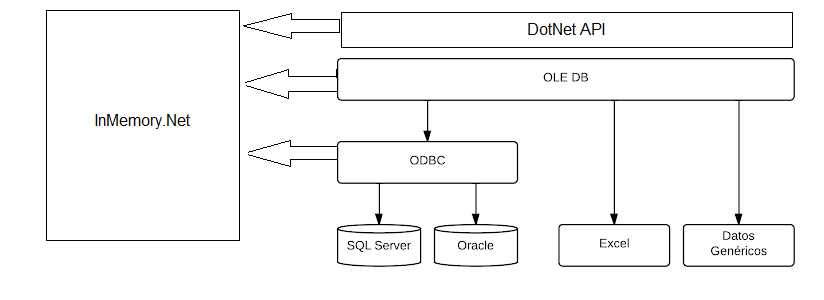
\includegraphics[width=\linewidth]{architecture_IRDB.png} % Figure image
	\caption{Arquitectura InMemory.NET} % Figure caption
	\label{irdb} % Label for referencing with \ref{irbd}
\end{figure}

\subsection{Tipo de almacenamiento utilizado}

Es una base de datos en memoria con almacenamiento columnar, diseñada para usar dentro del entorno Microsoft Dot Net. Aunque soporta la importación de tablas en modo no columnar, advierte funciona bien si solo hay unas pocas tablas involucradas. El modo NO COLUMNIZADO debe considerarse en este caso para estas tablas, ya que mantiene los datos en un estado sin columnas hasta que se emita el comando COLUMNIZE.

\subsection{Representación en memoria}

Para poder mantener tantos datos en la memoria como sea posible, los valores únicos dentro de cada columna se almacenan en una matriz de búsqueda. Otra matriz se utiliza como índice que corresponde con el valor real en la matriz de búsqueda.

\subsection{Mecanismos de compresión}

Cada valor se almacena una sola vez en lugar de varias veces. En el archivo físico comprimido, primero se guardan los valores únicos, seguidos del número requerido de bits utilizados para representarlo.

Cuando se carga en la memoria, se usan 8 bits (char) si el número de valores únicos es 255 o menos, 16 bits (ushort) si es 65535 o menos, de lo contrario, 32 bits (int).

\subsection{Particionamiento}

Al ser una base de datos con almacenamiento en columnas utiliza el particionamiento vertical. Aunque pude hacerlo horizontal, pero advierte disminuye el rendimiento en esas tablas.

\subsection{Operaciones DML}

\textbf{SELECT}: Es la piedra angular de cualquier consulta SQL. IRDB admite la sintaxis regular de selección de SQL.

\textbf{SELECT DISTINCT}: Es soportado pero está limitado internamente por el grupo por límites de cardinalidad.

\textbf{SELECT *}: Es soportado pero si se tiene columnas con caracteres no soportados, no se validarán y harán que la consulta se comporte mal. IRDB está diseñado para hacer consultas agregadas rápidamente. Las consultas no agregadas se ejecutarán y también continuará ejecutándose en su totalidad. Si selecciona una gran cantidad de registros las tablas con millones de registros no son un problema, pero si pasa una consulta que realiza un SELECT * desde una tabla con cientos de millones de registros, internamente va a través del proceso de creación de la tabla desde cero y columnizarla, posiblemente quedándose sin memoria.

\textbf{NOCACHE}: Como un refuerzo de rendimiento, IRDB crea tablas temporales cuando cree que las subconsultas podrían reutilizarse (por ejemplo, para JOIN anidados o donde se usan fechas dinámicas). La creación de estos archivos temporales se puede desactivar mediante la inclusión de NOCACHE.

\textbf{CACHE}: La creación las tablas temporales se puede desactivar mediante la inclusión de nocache = true en
archivo irdb.ini. La inclusión de la palabra clave CACHE en una declaración select, anula esta declaración por
usando caché.

\textbf{CASE STATEMENTS}: Suporta la siguiente estructura:
\begin{verbatim}
CASE WHEN logic_expression THEN SomeExpression
WHEN logic_expression2 THEN SomeExpression2
ELSE SomeOtherExpression END
\end{verbatim}

\textbf{COUNT}: Cuenta el número de filas de datos no nulos en la selección

\textbf{COUNT (DISTINCT)}: devuelve el número de valores distintos dentro de una tabla.

\textbf{SUM (DISTINCT)}: Cuando se le da un parámetro, realizará una suma única en esa columna. Si hay
valores duplicados solo se suman una vez. Con múltiples parámetros (que deben ser campos de la base de datos), encontrará los valores únicos, y suma la primera columna.

\textbf{OVER() / OVER (PARTITION BY )}: Permite que los valores que se devuelvan en función del resultado de una consulta secundaria dentro de una partición. Se utiliza principalmente con las funciones RANK () y DENSE\_RANK (). También se admiten SUM, MIN, MAX, ROW\_NUMBER.

\textbf{JOINS}: Revisar la sección de JOINS.

\textbf{GROUP BY, ORDER BY, HAVING}: Soporta las operaciones SQL.

\textbf{INTERSECT}: Devuelve las filas comunes entre dos instrucciones SELECT.

\textbf{EXCEPT}: Devuelve filas que están en una instrucción SELECT inicial, pero no en una consulta secundaria.

\textbf{UPDATE}: La actualización en IRDB funciona de manera similar a otras bases de datos como SQL Server. Si está consultando un actualiza en la versión actual en memoria solamente. Los cambios no se conservan en el disco.

\textbf{DELETE}: Hay soporte de eliminación momentánea. Si se emite el comando Delete, se elimina solo en la versión actual en memoria. Los cambios no son conservados en disco.

\subsection{Buffer diferencial, proceso de mezcla}

No hay información en la documentación referente a este tópico.

\subsection{Reconstrucción de tuplas}

Lo hace mediante ordenamiento natural en todas las columnas en ambas tablas, luego haciendo una fusión entre ellas para encontrar las filas comunes.

Implementa un algoritmo de clasificación al ordenar tablas grandes con grandes cantidades de columnas. Anteriormente utilizaba BigIntegers para clasificación. Sin embargo, era muy lento al ordenar grandes cantidades de columnas. Ahora sus algoritmos mejorados utilizan estructuras de longitudes de varios tamaños, y generan dinámicamente código y compilaciones para hacer la configuración de clasificación.

\subsection{Tipos de Joins}

Actualmente IRDB admite INNER y LEFT y CROSS, RIGHT JOINS y Full Joins. Se ejecutan mejor si tiene la tabla con la cardinalidad más alta primero, uniéndose contra las tablas con granularidad decreciente. Todos los joins son conducidas por la primera tabla que se asumen es la tabla principal. Soporta joins de hasta 50 dimensiones. Las consultas deben diseñarse sin bucles de unión y unirse de tal manera que las uniones fluyan desde la primera tabla o las tablas de nivel superior. Expresiones de los campos que involucran la misma tabla ahora son compatibles. Actualmente constantes por sí mismas no son compatibles.

\subsection{Logging / Recovery}

Almacena un registro lógico en el directorio principal. Proporciona un registro de los queries que se ejecutan y un desglose de los principales momentos de ejecución que se realizaron en la consulta.

\subsection{Respaldos}

La forma de obtener infomación es a través de la importación de algun ODBC u OLEDB. Por lo que el único respaldo posible es mediante la exportación desde IRDB como parte de un script IRDBIMPORT. Para esto las tablas deben ser importado dentro de la secuencia de comandos antes de exportar.

\begin{verbatim}
--import statement

SAVE TABLA <tableName> TO CSV <nombre de archivo>
\end{verbatim}

\subsection{Manejo de transacciones}

No cuenta con el soporte para transacciones.

\subsection{Cold / Hot store}

Se basa en hot storage. Ya que todo el tiempo la infomación se encuentra en memoria y esta diseñada para cargas de trabajo con muchas transacciones.

\subsection{Manejo de datos históricos}

No cuenta el soporte para datos históricos.

\newpage

\section{MySQL NDB Cluster}
Yann Le Lorier Bárcena
El DBMS de MySQL NDB Cluster es un sistema de administración de alta redundancia que está pensado para la computación distribuida (Oracle, s.f.)
\subsection{Arquitectura del DBMS}
La arquitectura del DBMS es la famosa three-tier architecture, separando en capas independientes los elementos entre el usuario y los datos en la BD.\\
Por otro lado, este DBMS está pensado como un sistema \textit{shared-nothing}, es decir que cada componente debe de tener su propio disco y memoria, por lo que la memoria compartida no es recomendable para este administrador.\\
En la figura \ref{mysqlarch}, podemos observar que la arquitectura del sistema está basada en un cluster de nodos interconectados de datos, el cual está también conectado a un servidor de administración. Como se puede acceder a los nodos de datos por medio de los nodos de SQL, cualquier dato cambiado en los nodos de datos, va a ser visible por cualquier nodo SQL. A su vez, los nodos SQL son los que se comunican con los clientes o APIs que realicen peticiones.
\begin{figure}
    \centering
    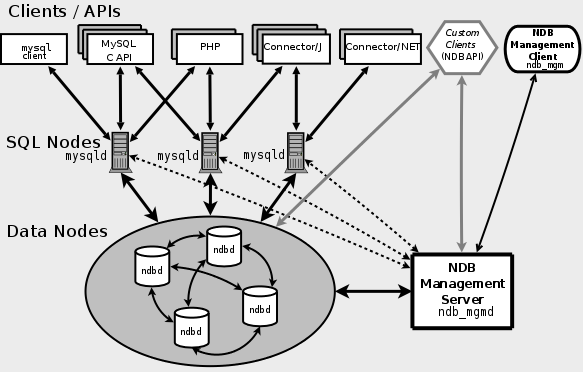
\includegraphics[width=0.4\linewidth]{mysqlndbarch.png}
    \caption{Arquitectura del MySQL NDB Cluster}
    \label{mysqlarch}
\end{figure}
\subsection{Tipo de almacenamiento utilizado}
\subsection{Representación en memoria}
La representación en memoria de cada una de las tablas se maneja de forma muy similar al MySQL tradicional. Por cada columna declarada en la definición de una nueva tabla, se suman el tamaño del tipo de dato que se está tomando en cuenta. Al agregar datos que no son 'NULLABLE', se ahorran algunos bytes por el overhead. Al agregar alguna PRIMARY KEY o algún valor UNIQUE, se tiene que sumar aproxmadamente 29 bytes por el índice hash.\\
Se trata, efectivamente, de un espacio considerable por registro, pero el hecho que existan los índices hash permiten una lectura muy rápida de los datos.

\begin{lstlisting}[language=sql]
    CREATE TABLE example (
  a INT NOT NULL,
  b INT NOT NULL,
  c INT NOT NULL,
  PRIMARY KEY(a),
  UNIQUE(b)
) ENGINE=NDBCLUSTER;
\end{lstlisting}
(Oracle, s.f., \cite{mysqlcomp})

\subsection{Mecanismos de compresión}
De acuerdo con la información extraída de la documentación sobre las definiciones de la creación del Cluster (Oracle, s.f., \cite{mysqlcomp}), dentro de la base de datos, existe un conjunto de variables que permiten comprimir:
\begin{itemize}
    \item los respaldos, y reducir el espacio utilizado en el disco, de 50\% o más. Se trata de una compresión que es equivalente al \textit{gzip--fast}. La elección entre tener o no activados los backups puede ser realizada para nodos individuales, o para todos los nodos.
    \item Se pueden también comprimir archivos de los \textit{local checkpoint files}, que utilizan una compresión que es de igual manera, equivalente al \textit{gzip--fast}
\end{itemize}


\subsection{Particionamiento}
Actualmente, el único algoritmo de particionamiento es el de hashing.\\
En MySQL NDB Cluster, el particionamiento se conoce como \say{Replicas}. Se dividen por los Clusters, que dividen la información a guardar, dependiendo de la partición que se le haya asignado. Todo este proceso es manejado automáticamente por el DBMS.\\
Es posible definir el particionamiento al nivel usuario, el NDBCLUSTER, que es usualmente definido automáticamente.\\
La \textit{Replicas} son copias de una partición del cluster. Cada nodo en un grupo de nodos contiene una réplica. Se trata de una relación 1 a n entre la réplica y el nodo, ya que por cada nodo, normalmente existen muchas réplicas, podemos observar un ejemplo en la imagen \ref{dosnodos}.

\begin{figure}
    \centering
    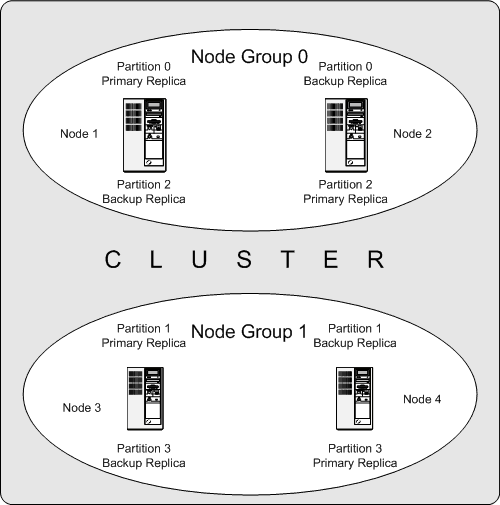
\includegraphics[width=0.4\linewidth]{replicas.png}
    \caption{Un Cluster con dos grupos de nodos}
    \label{dosnodos}
\end{figure}

\subsection{Operaciones DML}

\subsection{Buffer diferencial, proceso de mezcla}
NDB usa uno o más buffers de memoria para los eventos de los nodos que contienen la información. Para cada objeto NDB, existe un buffer que registra la información de los eventos que van sucediendo a nivel tabla, por lo que existe otro buffer que va registrando la información del esquema (Oracle, s.f., \cite{mysqlbuff}).\\
Estos buffers van imprimiendo su estado en el cluster log.
\subsection{Reconstrucción de tuplas}
\subsection{Tipos de Joins}
\subsection{Logging / Recovery}
\subsection{Respaldos}
Los respaldos de esta DBMS están basados en tres principales partes:
\begin{itemize}
    \item Metadata: Nombres y definiciones de todas las tablas de la base de datos
    \item Registros de tablas: la infomación que está guardada dentro de las tablas al momento de realizar el respaldo
    \item Registro de las transacciones: Se trata de un registro secuencial que tiene las 'instrucciones' para obtener la base de datos al momento del respaldo.
\end{itemize}
(Oracle, s.f. \cite{mysqlbackups})\\
Todos los nodos realizan cada uno el respaldo con las tres partes mencionadas anteriormente, las cuales se guardan en tres archivos en el disco del nodo:
\begin{itemize}
    \item \textit{<backup.id>.<node.id>.ctl} Toda la información de control y la metadata mencionada anteriormente
    \item \textit{<backup.id>.<node.id>.data} Un archivo que contiene toda la información con la que la tabla está rellenada. La información está fragmentada, dependiendo del nodo en cuestión, guardando información parcial de alguna tabla.
    \item \textit{<backup.id>.<node.id>.log} Un registro de transacciones a las que se les realizaron el \textit{commit}. De igual forma que el archivo de data, son diferentes registros por que la información está fragmentada.
\end{itemize}
\subsection{Manejo de transacciones}
Como lo dice su nombre, MySQL NDB Cluster, es un DBMS que está previsto para información fragmentada, en nodos de computación con su propia memoria y su propio disco.
En cada cluster de la base de datos, existe una tabla en particular que se llama \textit{cluster\_transactions} que es una tabla que muestra todas las transacciones que están ocurriendo en un cluster.\\
A continuación se describe la tabla \textit{cluster\_transactions} por columna:

\begin{center}
    \begin{tabular}{|c|c|}
        \hline
        node\_id & id del nodo que es el coordenador de la transacción \\
        \hline
        block\_instance & la instancia del bloque realizando la transacción \\
        \hline
        transid & id de la transacción \\
        \hline
        state & estado de operación\\
        \hline
        count\_operations & número de operaciones con llave primaria en la transacción \\
        \hline
        outstanding\_operations & operaciones que siguen siendo ejecutadas en los bloques locales de administración\\
        \hline
        inactive\_seconds & tiempo que ha transcurrido esperando al API \\
        \hline
        client\_node\_id & Id del nodo del cliente\\
        \hline
        client\_block\_ref & referencia del bloque del cliente\\
        \hline
    \end{tabular}
    \captionof{table}{descripción por columna de la tabla cluster\_transactions}
\end{center}

Analizando los inconvenientes del manejo de transacciones, podemos notar ciertos aspectos:
\begin{itemize}
    \item Soporte de sólamente las transacciones a las que se les hicieron \say{commit}, por lo que no se pueden ver las transacciones sin este proceso.
    \item Procesamiento intensivo de las transacciones por que cada una tiene que tener forzosamente la fase de \say{commit}
    \item No existen las transacciones parciales, ya que si se realiza un \say{rollback}, descarta desde el principio de la transacción, a diferencia de InnoDB, el cual permite el \say{rollback} de \say{statements} individuales.
\end{itemize}
(Oracle, s.f., \cite{mysqllimittrans})
\subsection{Cold / Hot store}
Mientras que en la documentación no existe una sección dedicada al Hot \& Cold storage, se menciona en la sección de backup troubleshooting. En esta sección habla que la recuperación de datos del backup es \say{hot} pero no lo es realmente en su totalidad, ya que explica que no existe soporte para lecturas repetidas (\textit{repeatable reads}), es decir que el DBMS no puede garantizar durante el proceso de respaldo que si intentamos leer la información nuevamente obtendremos el mismo resultado, por lo tanto existe información que es inconsistente durante este momento. (Oracle, s.f., \cite{mysqlhot})

\subsection{Manejo de datos históricos}

\newpage

\section{Raima}
Isaac Harari Masri

Raima Database Manager es un sistema de gestión de bases de datos relacionales desarrollado para aplicaciones de tiempo que requieren alto rendimiento, poco espacio y almacenamiento compacto.

Está diseñado para dispositivos con recursos limitados como internet de las cosas. el DBM sintetiza los datos en el dispositivo y se envían a la nube u otro sistema de base de datos detrás. El producto es capaz de ejecutarse en proceso con la aplicación, permitiendo que la aplicación se vuelva un servidor, o ejecutarse como una base de datos se cliente/servidor (más tradicional). Como resultado de la arquitectura flexible, logra un rendimiento rápido con transacciones cerradas.
\subsection{Arquitectura del DBMS}
Se obtiene más rendimiento cuando la base de datos se encuentra más cerca del consumidor. La arquitectura flexible de RDM le brinda una variedad de configuraciones. Use RDM en una aplicación cliente / servidor o punto a punto (\textit{embedded}) en casi cualquier combinación de hardware y software. RDM puede aprovechar al máximo la memoria, ya que el medio de almacenamiento principal y los datos persistentes pueden almacenarse en el disco. \cite{Rpdf1, Rarch}

En las siguiente imágene, se puede apreciar la arquitectura RDM gráficamente. Fig \ref{arqRaima}

\begin{figure}
	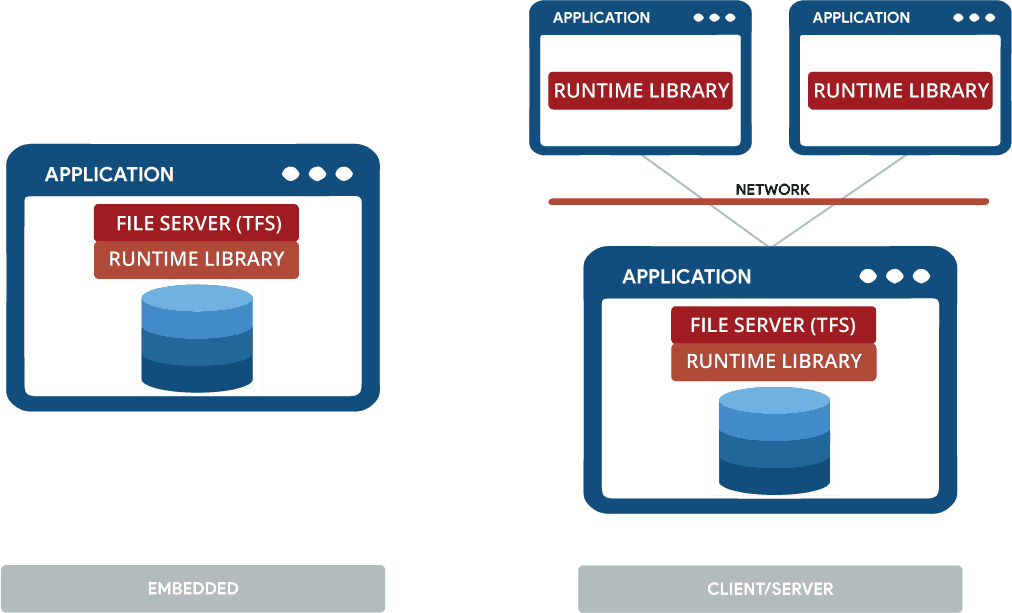
\includegraphics[width=\linewidth]{arq_1.png} % Figure image
	\caption{Arquitectura Raima} % Figure caption
	\label{arqRaima} % Label for referencing with \ref{irbd}
\end{figure}


\subsection{Tipo de almacenamiento utilizado}
El tipo de almacenamiento que utiliza Raima es \textit{object-oriented}. Una base de datos de objetos almacena datos complejos y relaciones entre datos directamente, sin asignar a filas y columnas relacionales. \cite{Rpdf1, Rarch}

\subsection{Representación en memoria}
Está dividido en dos componentes: \textit{runtime engine} y \textit{storage engine}:
\begin{itemize}
	\item Cuando \textit{runtime engine }necesita un objeto de la base de datos, se lo pide a \textit{storage engine. }Asimismo, cuando los cambios del \textit{runtime }son entregadosa \textit{storage }para que los guarde en una DB. \cite{Rinmemory}

	\item \textit{Storage }se puede ver como si fuera un repositorio de llave / valor. Las llaves son los id’s y los valores son el lugar de los objetos de la DB. \cite{Rinmemory}
\end{itemize}
\subsection{Mecanismos de compresión}
RDM implementa técnicas de compresión simples, así como la compresión LZMA opcional para reducir la cantidad de datos almacenados en el disco. \cite{Rover}
\subsection{Particionamiento}
Raima Utiliza particionamiento horizontal. Dado que se procesan en objetos, no se puede dividir verticalmente el mismo. Los datos se dividen según su llave primaria y en cuántos se quiera particionar. La aplicación va determinando en qué partición almacenar los registros. Al tener particiones, se puede trabajar en paralelo, lo que hace que la capacidad de procesamiento sea mucho mayor.
\subsection{Operaciones DML}
RDM se basa en las operaciones DML básicas de SQL.
Raima cuenta con las siguientes operaciones de lenguaje de manipulación de datos:\par
\begin{itemize}
    \item SELECT\par
	\item INSERT\par
	\item UPDATE\par
	\item DELETE\par
	\item LOCK\par
	\item ROLLBACK\par
	\item COUNT\par
	\item SUM\par
	\item AVG\par
	\item ORDER BY\par
	\item WHERE\par
\end{itemize}

En cualquier caso en donde se ejecuten comandos donde se inserten, actualicen o eliminen registros, de debe de ejecuta el comando \textit{COMMIT;} para que se guarde en la base de datos. En caso de no ejecutar el comando, cuando se cierre la DB y se vuelva a abrir, los cambios que se hicieron no se verán reflejados. \cite{Rsql, Rsort}
\subsection{Buffer diferencial, proceso de mezcla}
No hay información en la documentación referente a este tópico.
\subsection{Reconstrucción de tuplas}
No hay información en la documentación referente a este tópico.
\subsection{Tipos de Joins}
RDM admite LEFT, RIGHT, INNER, FULL OUTER y NATURAL JOIN. \cite{Rjoin}
\subsection{Logging / Recovery}
RDM cuenta con la replicación de data. Duplica la información de la tabla maestra a una tabla esclava. La parte sobresaliente es que la DB puede estar manejada en RDM o con un DBMS de terceros.

Los datos de estado almacenados en las tablas de la DB maestra, se replican a un sistema de control central que mantiene un historial permanente de todos los estados de los dispositivos. Asimismo, RDM tiene una biblioteca de notificación de cambio de base de datos que permite a la esclava acceder a los registros (logs) de la maestra.

En resumen, RDM implementa una copia de seguridad de la base de datos activa y crea un sistema de registros de transacciones con ACID con la recuperación automática de fallos. \cite{Rserv, Rwiki}
\subsection{Respaldos}
Alta disponibilidad al proporcionar la capacidad de hacer una copia de seguridad de los datos y al mismo tiempo proporcionar accesibilidad activa de lectura / escritura a los mismos datos. \cite{Rpdf2}
\subsection{Manejo de transacciones}
Raima define una transacción como un grupo de cambios en la base de datos que pueden ser tanto \textit{COMMIT} (se hagan permanentes) o \textit{ROLLED-BACK} (se decarten). Esto es necesario para mantener la coherencia lógica del contenido de la base de datos en caso de que el sistema falle (por ejemplo, falla de energía) en el medio de la transacción. Para inicar una transacción en Raima, se debe de escribir \textit{START TRANSACTION} y todos los cambios en la DB (INSERT, UPDATE, DELETE), ejecutados después del \textit{START}, no se ven reflejados a menos que la transacción termine. 

Para evitar \textbf{}{deadlocks} en una transacción que incluye varias sentencias, RDM permite hacer \textit{lock} de las tablas que se van a modificar. En caso de no hacerlo explícitamente (bloquear las tablas) después de \textit{START TRANSACTION}, se realizará automáticamente las solicitudes de bloqueo para cada sentencia. 

Si se llegara a producir un \textit{timeout} durante la ejecución de una instrucción de modificación de la base de datos, la respuesta correcta es hacer \textit{ROLLBACK}
a la transacción y luego reiniciarla. \cite{Rtrans}
\subsection{Cold / Hot store}
Raima tiene la habilidad de crear una copia de seguridad de la base de datos activa. \cite{Rserv}
\subsection{Manejo de datos históricos}
Como se mencionó anteriormente, RDM replica a un sistema de control central la información, el cual mantiene un historial permanente de todos los estados de los dispositivos. \cite{Rwiki}

\newpage

\section{Comparación entre DBMS}

\section{Conclusiones}

\begin{thebibliography}{99}
	\bibitem{mysqlbackups} Oracle. (n.d.). MySQL NDB Cluster Online Backup. Retrieved March 21, 2020, from https://dev.mysql.com/doc/mysql-cluster-excerpt/8.0/en/mysql-cluster-backup.html
	\bibitem{mysqltransactions} Oracle. (n.d.). MySQL NDB Cluster The ndbinfo cluster\_transactions Table. Retrieved March 21, 2020, from https://dev.mysql.com/doc/mysql-cluster-excerpt/8.0/en/mysql-cluster-ndbinfo-cluster-transactions.html
	\bibitem{mysqlhot} Oracle. (n.d.). MySQL NDB Cluster NDB Cluster Backup Troubleshooting. Retrieved March 21, 2020, from https://dev.mysql.com/doc/mysql-cluster-excerpt/8.0/en/mysql-cluster-backup-troubleshooting.html
	\bibitem{mysqllimittrans} Oracle. (n.d.). MySQL NDB Cluster Limits Relating to Transaction Handling in NDB Cluster. Retrieved March 21, 2020, from https://dev.mysql.com/doc/mysql-cluster-excerpt/5.7/en/mysql-cluster-limitations-transactions.html
	\bibitem{mysqlcomp} Oracle. (n.d.). MySQL NDB Cluster 8.0 :: 5.3.6 Defining NDB Cluster Data Nodes. Retrieved March 21, 2020, from https://dev.mysql.com/doc/mysql-cluster-excerpt/8.0/en/mysql-cluster-ndbd-definition.html
	\bibitem{mysqlpart} Oracle. (n.d.). MySQL 5.7 Reference Manual :: 21.1.2 NDB Cluster Nodes, Node Groups, Replicas, and Partitions. Retrieved March 21, 2020, from https://dev.mysql.com/doc/refman/5.7/en/mysql-cluster-nodes-groups.html
	\bibitem{mysqlbuff} Oracle. (n.d.). MySQL NDB Cluster 8.0 :: 7.7.3 Event Buffer Reporting in the Cluster Log. Retrieved March 22, 2020, from https://dev.mysql.com/doc/mysql-cluster-excerpt/8.0/en/mysql-cluster-logs-event-buffer.html
	\bibitem{inmemorynet} 
	In-Memory.NET,
    \\\texttt{https://inmemory.net/blog/}
    \bibitem{Rpdf1} Warren, W. (2016, enero). Raima Database Manager Version 14 Architecture and Features [PDF file]. \href{https://raima.com/wp-content/uploads/RDM-14.0-White-Paper.pdf}{\ul{https://raima.com/wp-content/uploads/RDM-14.0-White-Paper.pdf}}\par
	\bibitem{Rinmemory} Raima. (2019, November 18). In-Memory Database Questions and Answers. Retrieved March 19, 2020, from \href{https://raima.com/in-memory-database-qa/}{\ul{https://raima.com/in-memory-database-qa/}} \par
	\bibitem{Rarch} Raima. (2020, March 11). RDM Architecture. Retrieved March 19, 2020, from \href{https://raima.com/architecture/}{\ul{https://raima.com/architecture/}} \par
	\bibitem{Rover} Raima. (2020, March 11). Overview. Retrieved March 19, 2020, from \href{https://docs.raima.com/rdm/14_1/ug/learn/overview.htm}{\ul{https://docs.raima.com/rdm/14\_1/ug/learn/overview.htm}} \par
	\bibitem{Rsql} Raima. (2020, March 11). SQL Language Guide. Retrieved March 19, 2020, from \href{https://docs.raima.com/rdm/14_1/ug/sql/dbSQL.htm}{\ul{https://docs.raima.com/rdm/14\_1/ug/sql/dbSQL.htm}}\par
	\bibitem{Rsort} Raima. (2020, March 11). Sorting and Grouping Operations. Retrieved March 21, 2020, from \href{https://docs.raima.com/rdm/14_1/ug/sql/OptAccessSorting.htm}{\ul{https://docs.raima.com/rdm/14\_1/ug/sql/OptAccessSorting.htm}}\par
	\bibitem{Rserv} Raima. (n.d.). RDM Server. Retrieved March 21, 2020, from \href{https://raima.com/rdm-server/}{\ul{https://raima.com/rdm-server/}}\par
	\bibitem{Rwiki} Raima Database Manager. (2020, February 2). Retrieved March 21, 2020, from \href{https://en.wikipedia.org/wiki/Raima_Database_Manager}{\ul{https://en.wikipedia.org/wiki/Raima\_Database\_Manager}}\par
	\bibitem{Rpdf2} Johnson, P. (2008, enero). High Availability Using Raima Database Manager Server [PDF File]. \href{https://raima.com/wp-content/pdfs/whitepapers/high_availability_using_raima_database_manager.pdf}{\ul{https://raima.com/wp-content/pdfs/whitepapers/high\_availability\_using\_raima\_database\_manager.pdf}}\par
	\bibitem{Rjoin} Raima. (2020, March 11). Joins Involving Primary and Foreign Keys. Retrieved March 21, 2020, from \href{https://docs.raima.com/rdm/14_1/ug/sql/OptJoins.htm?Highlight=join}{\ul{https://docs.raima.com/rdm/14\_1/ug/sql/OptJoins.htm?Highlight=join}}\par
    \bibitem{Rtrans} Raima. (2020, March 11). Transactions. Retrieved March 21, 2020, from \href{https://docs.raima.com/rdm/14_1/ug/sql/TransactionLocking.htm}{\ul{https://docs.raima.com/rdm/14\_1/ug/sql/TransactionLocking.htm}}

\end{thebibliography}

\end{document}
